%
\section{Project Management}

\subsection{Project goals}

The goals of the project are:

\begin{itemize}
	\item Create, configure, manage and provide access to database
	\item Create a general library which enables management of information in the database
	\item Create a socket transfer server for communication purposes
	\item Create a sorting algorithm
	\item Manage a RFID reader
	\item Connect and control all software parts together
\end{itemize}

\subsection{Project Resources}

The hardware and software resources used in the development stage are described in the following subsections:

\subsubsection{Hardware Resources}
\begin{itemize}
	\item Configured MySQL server with Internet access or access on SDU domain
	\item Working RFID readers
\end{itemize}

\subsubsection{Software Resources}
\begin{itemize}
	\item MySQL database
	\item Microsoft Visual C\# tool
	\item .NET framework 3.5
	\item MySQL Connector Net 1.0.10
	\item Created simplified remote database configurator
	\item A RFID API .dll file provided by task 6
\end{itemize}

\subsection{Project Planning}

The duration of the project was approximately 19 weeks including design, implementation and documentation. A gant chart illustrating the entire project course is shown in figure \ref{fig:planning}, the chart describes tasks and marks the weeks denoted to that task. Project started on February 3 and finished at June 9.

\begin{figure}[h]
	\centering
		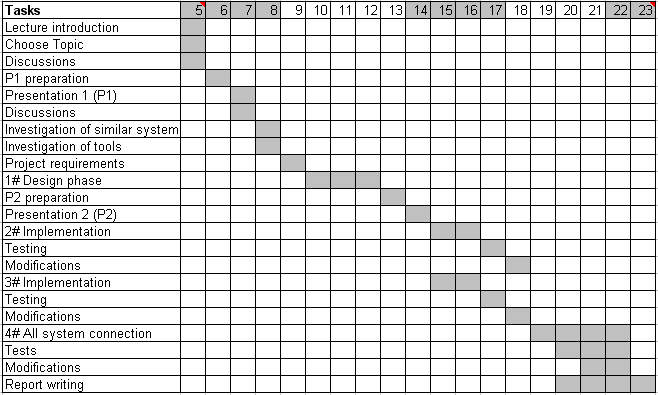
\includegraphics[scale=0.7]{planning}
	\caption{Work flow (Gant chart)}
	\label{fig:planning}
\end{figure}

\newpage
Work flow divided into four phases:

\begin{enumerate}
  \item 1\# Design – drawing diagrams, talking about similar systems and tools
  \begin{enumerate}
    \item Entity relation (ER) diagram
    \item Database connection class diagram (MySQL library)
    \item Sorting algorithm diagram
    \item Socket transfer protocol specifications
  \end{enumerate}
  \item 2\# Implementation
  \begin{enumerate}
    \item Configuration of database server
    \item Implementation of MySQL libraries
    \item Configuration of Web server
    \item Sorting algorithm
  \end{enumerate} 
  \item 3\# Implementation
  \begin{enumerate}
    \item Socket transfer server
    \item Sorting algorithm
  \end{enumerate}
  \item 4\# All system connection - all part connection into one software
  \begin{enumerate}
    \item Control RFID reader and provide access to subtask 4
    \item Connect RFID reader with sorting algorithm
    \item Connect RFID reader with socket transfer server
    \item Connect all together: RFID reader, MySQL library, socket transfer server and sorting algorithm
  \end{enumerate} 
\end{enumerate}

\newpage
\subsection{Work Responsibilities}


\begin{table}[h]
	\centering
    \begin{tabular}{ | p{3cm} | p{5cm} |}
    \hline
    \textbf{Responsibilities} &  \textbf{Tasks} \\ \hline
    All & Lecture introduction\\ \hline
    All & Choose Topic\\ \hline
    All & Discussions\\ \hline
    All & P1 preparation\\ \hline
    All & Presentation 1 (P1)\\ \hline
    All & Discussions\\ \hline
    All & Investigation of similar system\\ \hline
    All & Investigation of tools\\ \hline
    All & Project requirements\\ \hline
    All & 1\# Design phase\\ \hline
    All & P2 preparation\\ \hline
    All & Presentation 2 (P2)\\ \hline
    All & 2\# Implementation\\ \hline
    All & Testing\\ \hline
    All & Modifications\\ \hline
    All & 3\# Implementation\\ \hline
    All & Testing\\ \hline
    All & Modifications\\ \hline
    All & 4\# All system connection\\ \hline
    All & Testing\\ \hline
    All & Modifications\\ \hline
    All & Report writing\\ \hline
 		\end{tabular}
 		\caption{Work flow responsibilities}
	\label{tab:WorkFlow}
\end{table}


\subsection{Expectations}

To make sure that project will be delivered in time and all software function.
